\documentclass[12pt,a4paper]{report}

% ---------- Idioma y codificación ----------
\usepackage[spanish,es-noshorthands]{babel}
\usepackage[T1]{fontenc}
\usepackage{lmodern}

% ---------- Formato ----------
\usepackage[a4paper,margin=2.5cm]{geometry}
\usepackage{setspace}
\onehalfspacing
\usepackage{microtype}

% ---------- Matemática y unidades ----------
\usepackage{amsmath,amssymb}
\usepackage{siunitx}
\sisetup{output-decimal-marker={,}, per-mode=symbol}

% ---------- Figuras y tablas ----------
\usepackage{graphicx}
\graphicspath{{Figuras/}}
\usepackage{booktabs}
\usepackage{caption}
\usepackage{float}

% ---------- Bibliografía (IEEE, backend biber) ----------
\usepackage[backend=biber,style=ieee,sorting=none]{biblatex}
\addbibresource{referencias.bib}

% ---------- Enlaces (cargar al final) ----------
\usepackage[hidelinks]{hyperref}

% ---------- Datos del documento ----------
\title{Relevamiento técnico y normativo, estándares espaciales y técnicas de diseño de PCB orientadas a nanosatélites CubeSat}
\author{Agustín Mendes Rosa}
\date{\today}

\begin{document}

% ---------- Portada ----------
\begin{titlepage}
  \centering
  {\large Universidad Nacional de Córdoba\\
  Facultad de Ciencias Exactas, Físicas y Naturales\\
  Ingeniería Electrónica\par}
  \vspace{2cm}
  {\Large\bfseries Práctica Supervisada\par}
  \vspace{1cm}
  {\Large\itshape Relevamiento técnico y normativo, estándares espaciales y técnicas de diseño de PCB orientadas a nanosatélites CubeSat\par}
  \vspace{2cm}
  {\large Alumno: Agustín Mendes Rosa\par}
  \vspace{0.5cm}
  {\large Tutor de la entidad receptora: Mayco N. Orellano\\
  Tutor de carrera: Carlos R. Leguizamón\par}
  \vspace{0.5cm}
  {\large Laboratorio de Investigación Aplicada y Desarrollo (LIADE)\par}
  \vfill
  {\large Córdoba, \the\year\par}
\end{titlepage}

\tableofcontents
\listoffigures
\listoftables

% ---------- Contenido ----------
\chapter{Introducción}
\label{cap:introduccion}

% Contexto: proyecto del transponder CubeSat 1U en la facultad.
% Objetivo de la PS y relación con el Proyecto Integrador.
% Estructura del informe.

\chapter{Estándar CubeSat y especificación CDS}\label{cap:cds}

Este capítulo resume la \emph{CubeSat Design Specification} (CDS), Rev.~14.1, el documento que define las características físicas, eléctricas y operativas de un CubeSat. El objetivo es identificar qué restricciones impone el estándar al transponder de este proyecto, en particular a la cadena de amplificación y a la placa que la contiene. Salvo indicación contraria, los números de sección, valores y tablas citados provienen de la CDS~\cite{cds14}.

%--------------------------------------------------------------------
\section{Origen, propósito y alcance del estándar}\label{sec:cds-general}

El proyecto CubeSat nació en 1999 como una colaboración entre el Prof.~Jordi Puig-Suari (Cal Poly, San Luis Obispo) y el Prof.~Bob Twiggs (Laboratorio de Desarrollo de Sistemas Espaciales de Stanford). Buscaba reducir el costo y el tiempo de desarrollo, facilitar el acceso al espacio y sostener una alta frecuencia de lanzamientos~\cite[Sec.~1.1]{cds14}.

Un CubeSat es un satélite que adopta un tamaño y un factor de forma estandarizados, cuya unidad se denomina <<U>>. Un CubeSat de 1U es un cubo de \SI{10}{\centi\metre} de lado con una masa de hasta \SI{2}{\kilo\gram}~\cite[Sec.~1.1]{cds14}. El estándar cubre configuraciones de 1U a 12U y, como objetivo secundario, informa sobre los dispensadores (desplegadores) disponibles y sus interfaces.

La Rev.~14 (julio de 2020) reemplazó a la Rev.~13 y a la CDS de 6U, incorporó las configuraciones de 6U y 12U y pasó de un conjunto de requisitos rígidos a un documento más cercano a una guía de diseño. La Rev.~14.1 (febrero de 2022) eliminó la marca de borrador, actualizó la información de dispensadores y agregó aclaraciones en las secciones~2 y~3~\cite{cds14,cdsanuncio}. Según el sitio del programa CubeSat, la Rev.~14.1 es la versión vigente~\cite{cubesatinfo}.

\subsection{Jerarquía normativa y lenguaje de la especificación}\label{subsec:cds-jerarquia}

Los requisitos de la CDS están pensados para el diseño preliminar y se redactan de forma conservadora, para maximizar la compatibilidad con cualquier vehículo de lanzamiento. Una vez que el satélite está asignado a un lanzamiento, los requisitos del proveedor de lanzamiento (\emph{Launch Provider}) prevalecen sobre los de la CDS\@. Aun así, un diseño que cumpla la CDS debería cumplir la mayoría de los requisitos de los proveedores, y cada desvío reduce las posibilidades de encontrar una oportunidad de lanzamiento~\cite[Secs.~1.3 y 1.4]{cds14}.

La CDS distingue cuatro términos en sus especificaciones~\cite[Sec.~1.6]{cds14}:
\begin{itemize}
  \item \textbf{Shall} (<<deberá>>): requisito obligatorio, sujeto a verificación formal.
  \item \textbf{Should} (<<debería>>): recomendación fuerte. No cumplirla suele limitar las oportunidades de lanzamiento.
  \item \textbf{Will} (<<ocurrirá>>): evento que sucederá independientemente del desarrollador, y para el cual este debe estar preparado.
  \item \textbf{Note} (<<nota>>): consejo orientativo.
\end{itemize}

%--------------------------------------------------------------------
\section{Configuraciones y el CubeSat 1U}\label{sec:cds-configuraciones}

La Tabla~\ref{tab:cds-masa-cg} resume la masa típica máxima y los rangos admisibles del centro de gravedad (CG) para cada configuración, medidos desde el centro geométrico~\cite[Sec.~2.2.10 y 2.2.11, Tablas~1 y~2]{cds14}. La CDS aclara que se pueden evaluar masas mayores caso por caso, y que la masa admisible depende de las capacidades del dispensador.

\begin{table}[H]
  \centering
  \caption[Masa y centro de gravedad por configuración (CDS Rev.~14.1)]{Masa típica máxima y rango admisible del centro de gravedad por configuración (CDS Rev.~14.1, Tablas~1 y~2).}\label{tab:cds-masa-cg}
  \setlength{\tabcolsep}{5pt}
  \begin{tabular}{lcccc}
    \toprule
    Configuración & Masa [\si{\kilo\gram}] & X [\si{\centi\metre}] & Y [\si{\centi\metre}] & Z [\si{\centi\metre}] \\
    \midrule
    1U   & 2,00  & $\pm 2$   & $\pm 2$   & $\pm 2$   \\
    1,5U & 3,00  & $\pm 2$   & $\pm 2$   & $\pm 3$   \\
    2U   & 4,00  & $\pm 2$   & $\pm 2$   & $\pm 4{,}5$ \\
    3U   & 6,00  & $\pm 2$   & $\pm 2$   & $\pm 7$   \\
    6U   & 12,00 & $\pm 4{,}5$ & $\pm 2$ & $\pm 7$   \\
    12U  & 24,00 & $\pm 4{,}5$ & $\pm 4{,}5$ & $\pm 7$ \\
    \bottomrule
  \end{tabular}
\end{table}

Para el 1U, la masa máxima es de \SI{2}{\kilo\gram} y el CG debe quedar dentro de una caja de $\pm\SI{2}{\centi\metre}$ en cada eje. Esto es relevante para el diseño de la placa: la distribución de masas (batería, placas apiladas, PA con su disipador) afecta directamente el CG del satélite completo.

% Sugerencia: agregar en Figuras/ el dibujo del 1U del Apéndice B de la CDS y la Figura 2 (familia CubeSat).
% \begin{figure}[H]
%   \centering
%   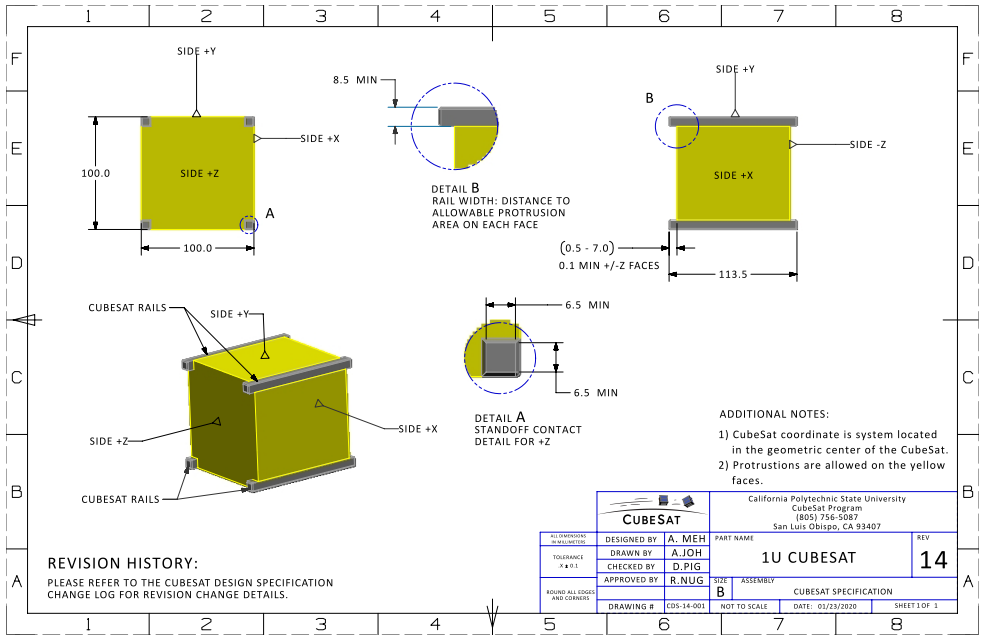
\includegraphics[width=0.8\textwidth]{cds_1u_dibujo.png}
%   \caption{Dibujo de especificación del CubeSat 1U (CDS Rev.~14.1, Apéndice~B)~\cite{cds14}.}
%   \label{fig:cds-1u}
% \end{figure}

%--------------------------------------------------------------------
\section{Especificaciones generales}\label{sec:cds-generales}

La sección~2.1 de la CDS reúne requisitos de seguridad y compatibilidad aplicables a todo el satélite~\cite[Sec.~2.1]{cds14}:

\begin{itemize}
  \item \textbf{Integridad:} ninguna parte puede desprenderse del satélite durante el lanzamiento, la eyección o la operación (2.1.1).
  \item \textbf{Pirotecnia, propulsión y materiales peligrosos:} deben cumplir el manual de seguridad de rango AFSPCMAN~91\nobreakdash-710, Vol.~3 (2.1.2, 2.1.3 y 2.1.6). Los sistemas de propulsión requieren al menos tres inhibiciones de activación (2.1.4). Este proyecto no incluye propulsión.
  \item \textbf{Baterías:} se recomienda considerar los límites de la FAA para baterías transportadas por pasajeros; por ejemplo, \SI{100}{\watt\hour} por batería de ion-litio de consumo (2.1.5).
  \item \textbf{Desgasificación (\emph{outgassing}):} los materiales deben tener una pérdida total de masa (TML) $\leq \SI{1,0}{\percent}$ y una masa volátil condensable colectada (CVCM) $\leq \SI{0,1}{\percent}$ (2.1.7). La CDS remite a la base de datos de materiales de la NASA\@.
  \item \textbf{Campo magnético:} los imanes pasivos deben limitar su campo a 0{,}5~gauss por encima del campo terrestre, fuera de la envolvente estática del satélite (2.1.8).
  \item \textbf{Venteo durante el ascenso:} el satélite debe admitir el venteo de ascenso con una relación volumen ventilable/área menor a \SI{50,8}{\metre} (2000 pulgadas) (2.1.9).
\end{itemize}

%--------------------------------------------------------------------
\section{Especificaciones mecánicas}\label{sec:cds-mecanicos}

Las dimensiones y características mecánicas se definen en los dibujos del Apéndice~B de la CDS\@. La CDS sugiere usar el procedimiento CIFP (\emph{CubeSat Inspection and Fit-check Procedure}), publicado en cubesat.org, para verificar el cumplimiento dimensional. Los requisitos de esta sección aplican a dispensadores que no usan el método de sujeción por pestañas (\emph{tabs}); los CubeSats con pestañas tienen requisitos propios, publicados por Planetary Systems Corporation (PSC)~\cite[Sec.~2.2]{cds14}.

\subsection{Sistema de coordenadas y dimensiones}\label{subsec:cds-coordenadas}

El origen del sistema de coordenadas está en el centro geométrico del CubeSat, y las dimensiones deben ajustarse al apartado correspondiente del Apéndice~B (2.2.1 y 2.2.1.1). La cara $-Z$ se inserta primero en el dispensador (2.2.2). Los separadores (\emph{standoffs}) de las caras $\pm Z$ evitan la interferencia con satélites vecinos y con la interfaz del dispensador (2.2.1.2)~\cite{cds14}.

Los valores dimensionales exactos del 1U (lado, altura total, tolerancias, posición de los rieles) están en el dibujo del Apéndice~B. \verificar{transcribir las cotas del 1U directamente del dibujo del Apéndice B de la CDS Rev.~14.1; el texto extraído no las incluye}

\subsection{Rieles y protuberancias}\label{subsec:cds-rieles}

\begin{itemize}
  \item Ningún componente de las caras laterales indicadas en el Apéndice~B puede sobresalir más de \SI{6,5}{\milli\metre} del plano del riel (2.2.3).
  \item Los elementos desplegables deben ser retenidos por el CubeSat y no por el dispensador (2.2.4).
  \item Los rieles deben tener un ancho mínimo de \SI{8,5}{\milli\metre}, medido desde el borde del riel hasta la primera protuberancia de cada cara (2.2.5).
  \item Los rieles deberían tener una rugosidad superficial menor a \SI{1,6}{\micro\metre} (2.2.6), lo que normalmente se cumple con un anodizado correcto, y sus bordes deberían estar redondeados con un radio de al menos \SI{1}{\milli\metre} (2.2.7).
  \item Los extremos de los rieles en las caras $\pm Z$ deben ofrecer una superficie de contacto mínima de $\SI{6,5}{\milli\metre} \times \SI{6,5}{\milli\metre}$ con los rieles de satélites vecinos (2.2.8). Si el CubeSat no comparte dispensador, el proveedor de lanzamiento puede eximir este requisito (2.2.8.1).
  \item Al menos el \SI{75}{\percent} del largo del riel debería estar en contacto con los rieles del dispensador; el \SI{25}{\percent} puede estar rebajado (2.2.9).
\end{itemize}

\subsection{Materiales y tratamiento superficial}\label{subsec:cds-materiales}

La estructura del CubeSat debería ser de aleación de aluminio. Típicamente se usan las aleaciones 7075, 6061, 6082, 5005 o 5052 tanto en la estructura como en los rieles (2.2.12). Las superficies externas de aluminio que contactan los rieles del dispensador (rieles y separadores) deben tener anodizado duro, para evitar la soldadura en frío dentro del dispensador (2.2.13)~\cite{cds14}.

\subsection{Mecanismo de separación}\label{subsec:cds-separacion}

Si el CubeSat comparte dispensador con otros, cada uno debe tener un mecanismo que favorezca la separación de sus vecinos (2.2.14). Como guía, la CDS recomienda un resorte de separación con fuerza máxima menor a \SI{6,7}{\newton} (1,5~lbf) y carrera mayor a \SI{2,5}{\milli\metre} (0,1~pulgadas). Un resorte demasiado fuerte puede superar al resorte del dispensador y producir una separación impredecible; uno demasiado débil puede no alcanzar a separarlos lo suficiente (2.2.14.1). El mecanismo no debe sobresalir del nivel del separador en configuración estibada (2.2.14.2) y no es necesario si el satélite no comparte dispensador (2.2.14.4)~\cite{cds14}.

%--------------------------------------------------------------------
\section{Especificaciones eléctricas}\label{sec:cds-electricos}

La sección~2.3 define las características de seguridad eléctrica que deben cumplirse con cualquier dispensador~\cite[Sec.~2.3]{cds14}.

\subsection{Estado apagado y conmutador de despliegue}\label{subsec:cds-despliegue}

El sistema de potencia del CubeSat debe estar apagado desde la entrega al vehículo de lanzamiento hasta el despliegue en órbita (2.3.1), de modo de impedir la activación de funciones alimentadas. Esas funciones incluyen subsistemas como el procesamiento y manejo de datos (C\&DH), la comunicación por RF, la determinación y control de actitud y la actuación de mecanismos desplegables. El sistema de potencia incluye las baterías y las celdas solares (2.3.1.1).

El satélite debe tener al menos un conmutador de despliegue (\emph{deployment switch}) que esté accionado mientras el satélite está integrado en el dispensador (2.3.2). En estado accionado debe desconectar eléctricamente el sistema de potencia de las funciones alimentadas (2.3.2.1) y debería quedar al nivel de la superficie externa o por debajo, para no dañar la superficie de contacto (2.3.2.3). Si el conmutador pasa de accionado a liberado y vuelve a accionarse, el satélite debe reiniciarse al estado previo al lanzamiento, incluidos los temporizadores de transmisión y despliegue (2.3.2.4)~\cite{cds14}.

\subsection{Relojes de tiempo real, pin RBF y baterías}\label{subsec:cds-rbf}

\begin{itemize}
  \item \textbf{RTC:} se permiten relojes de tiempo real si cumplen lo anterior, están aislados del sistema de potencia principal, operan a menos de \SI{320}{\kilo\hertz} y tienen la corriente limitada a menos de \SI{10}{\milli\ampere} (2.3.3).
  \item \textbf{Pin RBF (\emph{Remove Before Flight}):} el satélite debe incluir un pin que corte toda la alimentación mientras esté insertado (2.3.5). Debe sobresalir como máximo \SI{6,5}{\milli\metre} de la superficie del riel (2.3.5.2). Si el dispensador no tiene puertos de acceso, el RBF debe retirarse antes de la integración (2.3.5.1), por lo que conviene considerar esto en la secuencia de encendido y arranque (2.3.4.1).
  \item \textbf{Baterías:} el satélite debe incorporar protección de circuito para carga y descarga, que evite el desbalance de celdas. Las celdas modificadas o sin certificación UL requieren documentación y ensayos adicionales (2.3.6).
\end{itemize}

\subsection{Inhibiciones de RF y de desplegables}\label{subsec:cds-inhibiciones}

Este apartado es el más relevante para un transponder. La CDS exige \textbf{al menos tres inhibiciones independientes} para impedir una transmisión de RF involuntaria (2.3.7). Una inhibición es un dispositivo físico entre una fuente de energía y un peligro, y un temporizador \emph{no} cuenta como inhibición independiente (2.3.7.1 y 2.3.7.2). Algunos proveedores de lanzamiento solo exigen una o dos según la potencia de RF de salida, pero la CDS recomienda fuertemente usar tres, porque reduce la documentación y los análisis requeridos (2.3.7.3). De forma análoga, se exigen al menos tres inhibiciones independientes para impedir la liberación involuntaria de estructuras desplegables, como antenas o paneles solares (2.3.8)~\cite{cds14}.

%--------------------------------------------------------------------
\section{Especificaciones operativas}\label{sec:cds-operativos}

La sección~2.4 recoge obligaciones legales y de seguridad hacia otros satélites~\cite[Sec.~2.4]{cds14}:

\begin{itemize}
  \item \textbf{Licencias de radiofrecuencia:} los operadores deben obtener y documentar las licencias de uso de frecuencias (2.4.1). Para frecuencias de radioaficionados se requiere la coordinación de frecuencias de la IARU (2.4.1.1). Además, el satélite debe cumplir los acuerdos y restricciones de licencias de radio de su país, y la CDS remite a la UIT para determinar las aprobaciones necesarias (2.4.2).
  \item \textbf{Escombros orbitales:} el diseño debe ser conforme a NPR~8715.6 (2.4.3). Cualquier componente que reingrese debe hacerlo con una energía menor a \SI{15}{\joule} (2.4.3.1).
  \item \textbf{Temporización post-despliegue:} los desplegables deben esperar al menos \SI{30}{\minute} tras la activación de los conmutadores de despliegue (2.4.4). El satélite no debe generar ni transmitir ninguna señal antes de \SI{45}{\minute} desde el despliegue en órbita (2.4.5), aunque puede encenderse inmediatamente después del despliegue (2.4.5.1).
  \item \textbf{Verificación de ajuste:} se realizan al menos una verificación de encaje (\emph{fit check}) y otra final antes de la integración al dispensador (2.4.7).
\end{itemize}

%--------------------------------------------------------------------
\section{Requisitos de ensayo}\label{sec:cds-ensayos}

La CDS indica que los niveles y requisitos de ensayo son específicos de cada misión y los define el proveedor de lanzamiento. Típicamente se realizan ensayos de vibración aleatoria, de horneado en vacío térmico (\emph{thermal vacuum bakeout}) para asegurar la desgasificación de componentes, de choque (normalmente no requerido para CubeSats) y una inspección visual con mediciones críticas según el CIFP~\cite[Sec.~3]{cds14}. Si el entorno del lanzador se desconoce, pueden usarse como referencia GSFC-STD-7000A y SMC-S-016, aunque sus niveles no garantizan cubrir todos los lanzadores. El satélite puede pasar por una campaña de calificación o de \emph{protoflight}; en este último caso, el modelo de vuelo no debe desarmarse ni modificarse después del ensayo (3.5)~\cite{cds14}.

La CDS \emph{no} fija niveles numéricos de vibración ni de choque: remite al proveedor de lanzamiento. Esto es importante para el diseño de la placa (componentes pesados, sujeción de conectores, fijación del PA), porque los niveles reales se conocerán recién al definirse el lanzamiento.

%--------------------------------------------------------------------
\section{Dispensadores}\label{sec:cds-dispensadores}

El dispensador lleva los CubeSats y es la interfaz con el vehículo de lanzamiento. Todos los dispensadores actuales adhieren a uno de dos sistemas de sujeción: el de \textbf{rieles}, desarrollado por Cal Poly para el P-POD, y el de \textbf{pestañas}, desarrollado por PSC\@. En ambos casos, un resorte impulsa una placa empujadora que eyecta al satélite. La CDS aclara que no se espera que un mismo CubeSat sea compatible con ambos tipos~\cite[Sec.~4]{cds14}.

La CDS lista, en su Tabla~3, los dispensadores disponibles (P-POD, ISIPOD, 6-POD, QuadPack, J-SSOD, CSD de PSC, NLAS de Tyvak, entre otros) con sus opciones: puertos de acceso, masa adicional, longitud extendida, protuberancias extendidas, puerto de energía/datos, purga gaseosa y volumen adicional en $-Z$ (\emph{tuna can})~\cite[Sec.~5]{cds14}. Advierte además que diseñar el satélite para una característica que no está en todos los dispensadores restringe las oportunidades de lanzamiento.

%--------------------------------------------------------------------
\section{Implicancias para el transponder}\label{sec:cds-implicancias}

La Tabla~\ref{tab:cds-impacto} relaciona las especificaciones de la CDS con las decisiones de diseño de la cadena de amplificación y de la placa del transponder. La columna de impacto es una interpretación de este trabajo, no un requisito de la CDS\@.

\begin{table}[H]
  \centering
  \caption[Especificaciones de la CDS con impacto sobre el transponder]{Especificaciones de la CDS con impacto sobre el transponder (la columna <<Impacto>> es una interpretación propia).}\label{tab:cds-impacto}
  \small
  \begin{tabular}{@{}>{\raggedright\arraybackslash}p{2.2cm}>{\raggedright\arraybackslash}p{5.6cm}>{\raggedright\arraybackslash}p{7.2cm}@{}}
    \toprule
    Sección & Contenido & Impacto sobre el diseño \\
    \midrule
    2.3.7 & Al menos tres inhibiciones de RF independientes; un temporizador no cuenta. & Prever un mecanismo físico que corte la alimentación o la señal de la cadena de amplificación. Definir con el equipo de sistema cuáles inhibiciones recaen en este subsistema. \\
    2.3.1 y 2.3.2 & Sistema apagado hasta el despliegue; conmutador que desconecta la potencia de las funciones alimentadas. & El transponder no debe quedar alimentado con el conmutador accionado. Revisar la distribución de alimentación en la placa. \\
    2.4.5 & Sin transmisión hasta \SI{45}{\minute} después del despliegue. & El PA debe permanecer inhibido durante ese período. \\
    2.4.1 y 2.4.2 & Licencia y coordinación de frecuencias (IARU para radioaficionados). & Las bandas de operación (VHF/UHF) y la potencia de salida deben ser consistentes con la licencia que se tramite. \\
    2.1.7 & TML $\leq \SI{1,0}{\percent}$ y CVCM $\leq \SI{0,1}{\percent}$. & Condiciona la elección de sustrato, máscara, adhesivos y componentes. \\
    2.2.10 y 2.2.11 & Masa de hasta \SI{2}{\kilo\gram} y CG dentro de $\pm\SI{2}{\centi\metre}$ en el 1U. & Limita la masa del PA y su disipación, y la ubicación de componentes pesados. \\
    2.2.3 y 2.2.5 & Protuberancias de hasta \SI{6,5}{\milli\metre} y ancho mínimo de riel de \SI{8,5}{\milli\metre}. & Restringe la altura de conectores y componentes que sobresalgan. \\
    2.1.8 & Imanes pasivos limitados a 0{,}5~gauss. & Cuidado con componentes magnéticos (inductores, relés, aisladores/circuladores de ferrita). \\
    3 & Ensayos de vibración y térmico-vacío definidos por el proveedor de lanzamiento. & Elegir componentes y fijaciones aptos para vibración y vacío. \\
    \bottomrule
  \end{tabular}
\end{table}

La CDS no fija un presupuesto de potencia ni tensiones de bus: esos valores dependen del subsistema de energía del satélite que desarrolla la facultad. Tampoco se menciona el estándar PC/104 en el texto de la especificación, de modo que el apilamiento de placas es una decisión de diseño del proyecto, que se estudia en el Capítulo~\ref{cap:pc104}.

%--------------------------------------------------------------------
\section{Síntesis}\label{sec:cds-sintesis}

La CDS Rev.~14.1 define una envolvente mecánica y un conjunto de salvaguardas eléctricas y operativas que cualquier CubeSat debe respetar para ser aceptado en un lanzamiento. Para el transponder del proyecto, los puntos de mayor impacto son las inhibiciones de RF, el retardo de \SI{45}{\minute} para transmitir, la licencia de frecuencias, los límites de masa y de centro de gravedad del 1U, y los criterios de materiales de bajo \emph{outgassing}. Los requisitos del proveedor de lanzamiento prevalecen sobre los de la CDS, por lo que los valores aquí presentados deben tomarse como el punto de partida de diseño.
\chapter{Arquitectura de apilamiento PC/104}\label{cap:pc104}

Este capítulo estudia el formato PC/104, que se usa como estándar para apilar placas dentro de un CubeSat. El objetivo es obtener las dimensiones de la placa, los agujeros de fijación, los conectores y los pines que condicionan el diseño del PCB del transponder.

\section{El estándar PC/104 y su rol en los CubeSat}\label{sec:pc104-general}

PC/104 es una familia de estándares para computadoras embebidas, definidos por el PC/104 Embedded Consortium, que especifican tanto un factor de forma como un bus. El bus ISA (\emph{Industry Standard Architecture}) original combinaba dos buses de datos: el PC (8 bits) de 64 pines, que maneja señales de datos, y el PC/AT (16 bits) de 40 pines, que suma más lineas de interrupción y DMA\@. La suma de los pines da 104, lo que le da el nombre a la familia de estándares~\cite{pc104v24,pc104wiki}. 

Su principal característica es el apilamiento: los módulos se montan unos sobre otros mediante un conector de bus que atraviesa la placa y separadores en las cuatro esquinas, sin necesidad de \emph{backplane} (placa base común)~\cite{pc104v24}.

\begin{figure}[H]
  \centering
  \begin{subfigure}[t]{0.48\textwidth}
    \centering
    \fbox{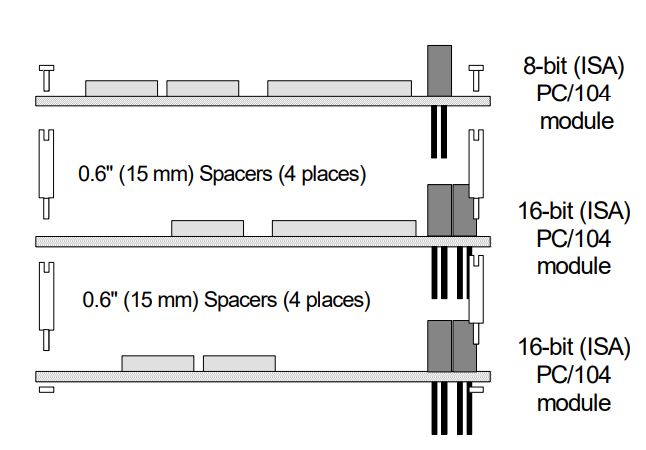
\includegraphics[width=\textwidth]{apilamiento.png}}
    \caption{}\label{fig:apilamiento-a}
  \end{subfigure}\hfill
  \begin{subfigure}[t]{0.48\textwidth}
    \centering
    \fbox{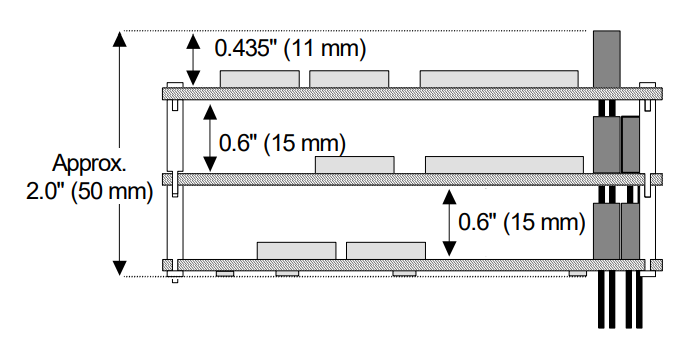
\includegraphics[width=\textwidth]{apilamiento2.png}}
    \caption{}\label{fig:apilamiento-b}
  \end{subfigure}
  \caption{Apilamiento de módulos típico. Fuente:~\cite[Sec. 2.2]{pc104v24}.}\label{fig:apilamiento}
\end{figure}


\subsection{Factor de forma frente a bus}\label{subsec:pc104-formafactor}

La especificación PC/104 define como obediente (\emph{compliant}) a los dispositivos que cumplen todos los aspectos no opcionales, sean mecánicos o eléctricos, y como \emph{bus-compatible} a los que no respetan las dimensiones pero proveen un conector de bus que sí cumple la especificación~\cite[Sec.~4]{pc104v24}. En el ámbito CubeSat, la tienda CubeSatShop aclara que la mayoría de los productos son <<bus-compatible>>: algunas especificaciones difieren levemente del estándar (como la posición del conector).

Cuando se habla de que un CubeSat usa PC/104, en la práctica se refiere a la forma de la placa, la ubicación de los agujeros de montaje y el conector físico de $2\times 2\times 26$ pines. Los CubeSats no adoptan la señalización ni los protocolos del estándar PC/104, y la asignación de cada pin queda a criterio del fabricante~\cite{cubesatshopfaq}. 

Un mensaje en una lista de correo de AMSAT ilustra el problema desde el lado del diseñador los conectores ocupan espacio, y no siempre se usa la cantidad completa de pines, además de que agregan masa de un solo lado, lo que desplaza el centro de masa. Señala también que los diseños de AMSAT usan varios buses a la vez (RS232, I2C, CAN y señales discretas), con interfaces, tensiones y firmware distintos~\cite{amsatpc104}. 

La propia CDS no menciona el PC/104 en su texto; es una convención de la industria, y no un requisito de lanzamiento.

%--------------------------------------------------------------------
\section{Dimensiones geométricas y orificios de fijación}\label{sec:pc104-dimensiones}

Las Figuras~\ref{fig:pc104-dim-16} y~\ref{fig:pc104-dim-8} resume la geometría del módulo según el Apéndice~A de la especificación PC/104 v2.4~\cite{pc104v24}. Las versiones de 8 y 16 bits tienen el mismo patrón de agujeros desde la versión 2.1 de la especificación~\cite{pc104v24}.

\begin{figure}[H]
  \centering
  \fbox{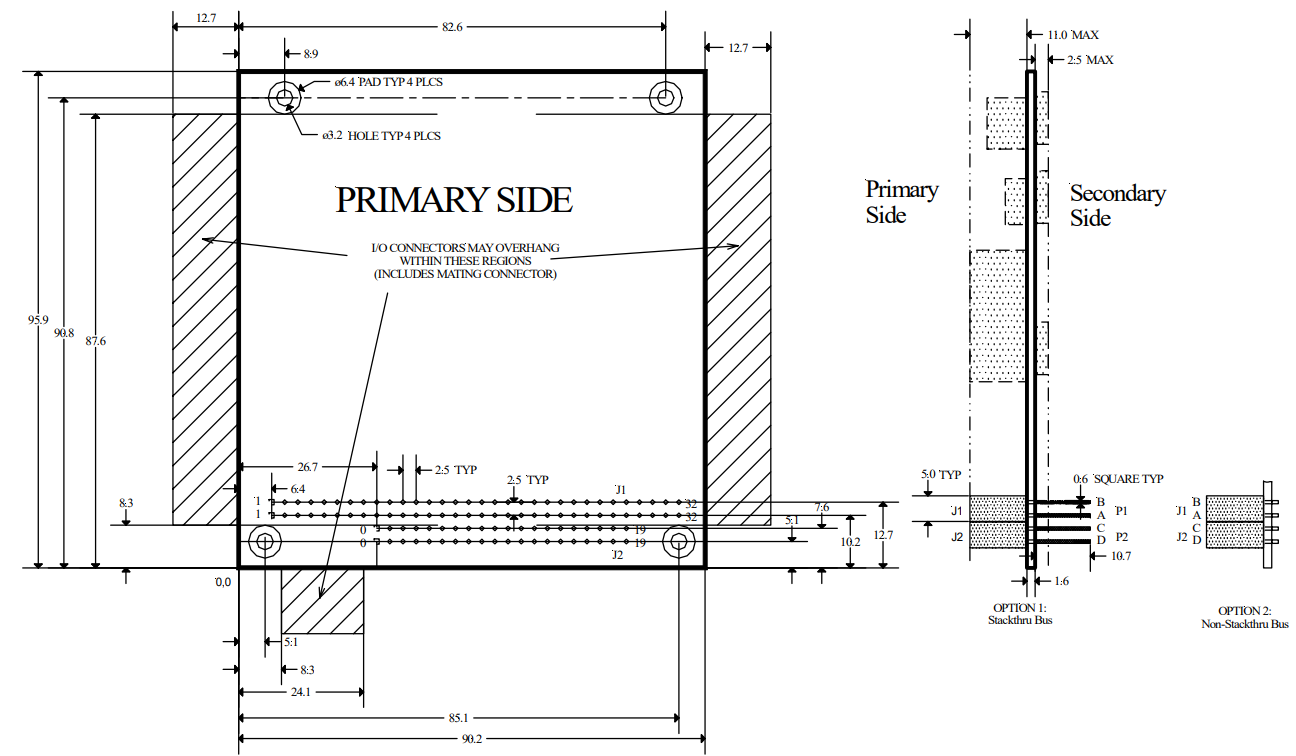
\includegraphics[width=0.98\textwidth]{pc104_dim_16.png}}
  \caption{Dimensiones de módulo de PC/104 16-bit en milímetros.}\label{fig:pc104-dim-16}
\end{figure}

\begin{figure}[H]
  \centering
  \fbox{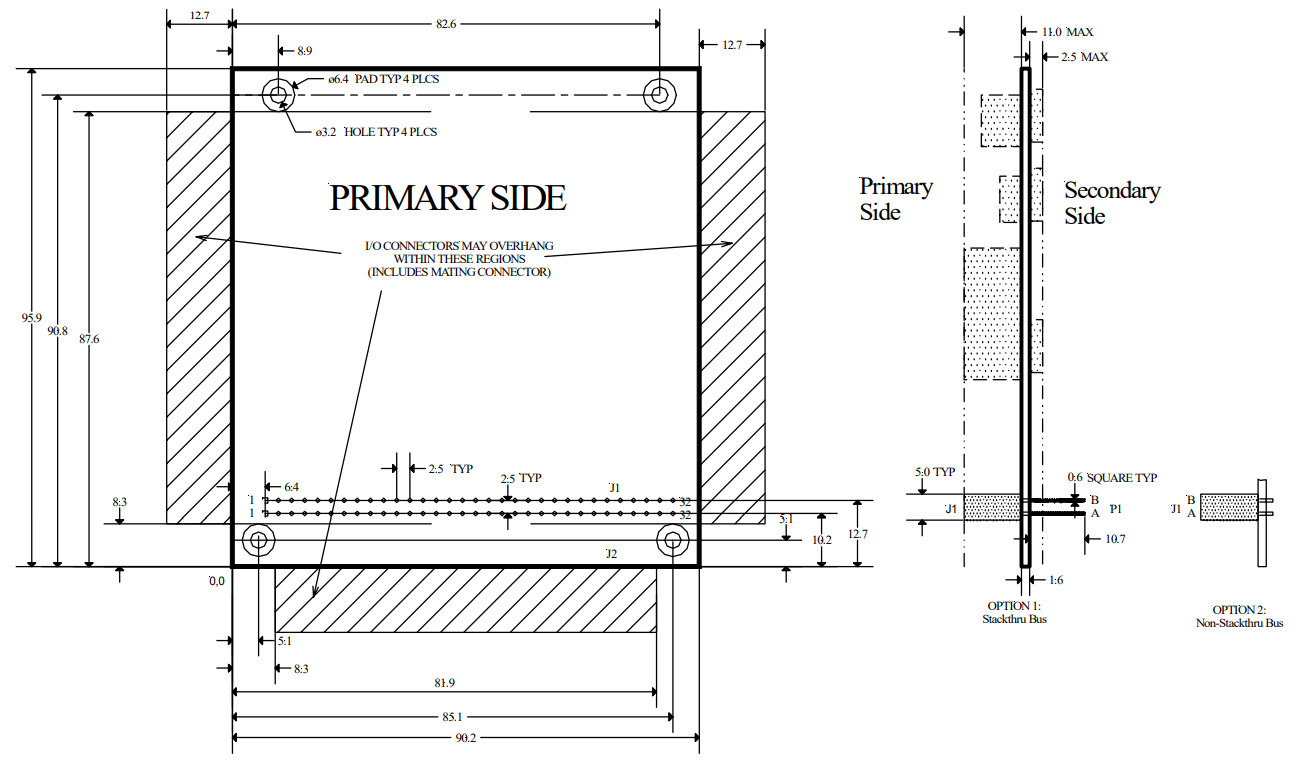
\includegraphics[width=0.98\textwidth]{pc104_dim_8.png}}
  \caption{Dimensiones de módulo de PC/104 8-bit en milímetros.}\label{fig:pc104-dim-8}
\end{figure}

La especificación ofrece dos opciones de bus según si los conectores P1 y P2 atraviesan el módulo (\emph{stackthrough}) o no. Si se combinan módulos de 8 y 16 bits en una pila, los de 16 bits deben ir por debajo de los de 8 bits, como puede observarse en la Figura~\ref{fig:apilamiento}~\cite[Sec.~2.2]{pc104v24}.

\subsection{Variaciones en placas para CubeSat}\label{subsec:pc104-variaciones}

Las placas comerciales para CubeSat respetan el patrón de agujeros, pero el contorno varía levemente entre fabricantes. La Tabla~\ref{tab:ejemplos} compara dos placas de prototipado de empresas distintas, aunque ambas son compatibles con los agujeros de fijación y la ubicación de los conectores~\cite{pumpkinprotoboard,ardusat}.

\begin{table}[H]
  \centering
  \begin{tabular}{@{}llccc@{}}
    \toprule
    Empresa & Modelo & Ancho [\si{\milli\metre}] & Largo [\si{\milli\metre}] & Masa [\si{\gram}] \\
    \midrule
    Pumpkin & Prototyping / Breadboard Module & \num{96} & \num{90} & \num{43}~\cite{pumpkinprotoboard} \\
    ArduSat & Prototyping Module & \num{95,45} & \num{90,3} & \num{42}~\cite{ardusat} \\
    \bottomrule
  \end{tabular}
  \caption{Dimensiones y masa de placas de prototipado comerciales para CubeSat.}\label{tab:ejemplos}
\end{table}

También se tienen alturas máximas por sobre y por debajo de la placa, lo cual tiene consecuencias de diseño: la altura máxima de componentes están acotados, tanto por la separación de la pila como por la altura de los conectores. Los valores concretos dependen del fabricante del resto de la pila y deben acordarse con el equipo que arma el satélite.

%-------------------------------------------------
\section{Conectores}\label{sec:pc104-conectores}

\subsection{Conector PC/104 original}\label{subsec:pc104-conector-orig}

El bus PC/104 tiene dos conectores: P1/J1, de 64 pines (2 filas de 32: A y B), y P2/J2, de 40 pines (2 filas de 20: C y D), que suman las 104 conexiones del nombre~\cite[Sec.~1 y Apéndice~B]{pc104v24}. Los módulos de 8 bits solo necesitan el conector P1. La Tabla~\ref{tab:pc104-conector-esp} resume las especificaciones del conector del Apéndice~D de la especificación.

\begin{table}[H]
  \centering
  \begin{tabular}{@{}>{\raggedright\arraybackslash}p{5.5cm}>{\raggedright\arraybackslash}p{9cm}@{}}
    \toprule
    Parámetro & Característica \\
    \midrule
    Capacidad de corriente & \SI{1}{\ampere} continuo por pin \\
    Resistencia de contacto & $<\SI{30}{\milli\ohm}$ \\
    Rigidez dieléctrica & \SI{1000}{\volt} (CA) \\
    Resistencia de aislación & $\geq \SI{5000}{\mega\ohm}$ \\
    Temperatura de operación & de \SI{-55}{\celsius} a \SI{+85}{\celsius} \\
    Durabilidad & 50 ciclos mínimo \\
    Carcasa & Termoplástico de alta temperatura, UL 94-V0 \\
    Contacto & Bronce fosforoso \\
    \bottomrule
  \end{tabular}
  \caption{Especificaciones del conector de bus PC/104 (v2.4, Apéndice~D).}\label{tab:pc104-conector-esp}
\end{table}

\subsection{Conector del CubeSat Kit Bus}\label{subsec:pc104-cskb}

En los CubeSats se usa un conector propio, el \emph{CubeSat Kit Bus} (CSKB), que consiste en dos conectores, H1 y H2, de $2\times2\times 26$ pines cada uno (104 pines en total), ubicados en el mismo lugar que los conectores PC/104 sobre la placa~\cite{pumpkinmb,cubesatshopfaq,amsatpc104}.
Pumpkin especifica una corriente máxima de \SI{3}{\ampere} por pin del conector CSKB~\cite{pumpkinmb}, frente a \SI{1}{\ampere} del conector PC/104 original (Tabla~\ref{tab:pc104-conector-esp}).

%--------------------------------------------------------------------
\section{Distribución de pines}\label{sec:pc104-pines}

Las señales del PC/104 original son idénticas a las del bus ISA, las únicas que importan son las de alimentación y masa.

La asignación de pines de H1 y H2 no forma parte de ningún estándar formal: es la convención de Pumpkin, que otros fabricantes siguieron con variantes~\cite{amsatpc104}. Por ejemplo, la hoja de opciones de la computadora a bordo CubeComputer (CubeSpace) permite configurar algunos pines (bus I2C secundario en H1.21 y H1.23, alimentación de 3,3\,V siempre activa en H2.27 y H2.28)~\cite{cubespace}. 

La Sección \emph{CubeSat Kit Bus PIN DESCRIPTIONS} de la hoja del datos del modelo \emph{Single Board Computer Development Platform} de Pumpkin muestra la función de cada uno de los pines del conector~\cite{}.

% Haceme una cita de esto si no está: https://www.pumpkininc.com/space/datasheet/710-00297-E_DS_DB.pdf

\chapter{Técnicas de layout de PCB para RF y aplicaciones espaciales}
\label{cap:layout}

\section{Líneas de transmisión planares}
\label{sec:layout-lineas}

\chapter{Gestión térmica y apantallamiento electromagnético}\label{cap:termica-emi}

Este capítulo trata dos problemas que el layout de RF del Capítulo~\ref{cap:layout} deja abiertos. El primero es dónde va el calor que disipa la placa cuando no hay aire, y el segundo es cómo evitar que la cadena filtro--amplificador--filtro se acople consigo misma o con el resto del satélite. Como en el capítulo anterior, los números marcados como cálculo propio se obtuvieron con fórmulas de las fuentes citadas, con las hipótesis que se indican en cada caso. No se compararon con simulaciones ni con mediciones, de modo que son órdenes de magnitud para decidir el diseño y no valores de verificación.

\verificar{la potencia que disipará la etapa de amplificación del PI y su temperatura máxima de unión. En el capítulo se usan como ejemplo los \SI{2}{\watt} de un amplificador de otro CubeSat~\cite{guerra18}, que no son datos del proyecto}

%--------------------------------------------------------------------
\section{Transferencia de calor en vacío}\label{sec:termica}

\subsection{Mecanismos y planteo}\label{sec:termica-mecanismos}

En órbita no hay convección: el calor se mueve por conducción dentro del satélite y por radiación hacia el exterior~\cite{nasasoa}. El balance de energía del satélite incluye las cargas solar, de albedo y de emisión planetaria, más el calor generado y el almacenado, y se cierra con la radiación emitida~\cite{nasasoa}. Un CubeSat tiene poca masa térmica, superficie y volumen limitados, poca potencia disponible para control activo y electrónica apilada muy cerca, de modo que disipar potencia es difícil y los componentes quedan muy acoplados entre sí~\cite{nasasoa}. En los CubeSat suele no haber lugar para aislación multicapa, por lo que la solución térmica es en gran parte un problema de recubrimientos~\cite{nasasoa}. Esto último es una decisión de la estructura del satélite y no de la placa del PI\@.

Para el diseño de la placa interesa el tramo interior: el camino del calor desde el componente hasta la estructura (Figura~\ref{fig:termica-red}). Cada tramo se modela como una resistencia térmica en serie, y la temperatura del componente es la de la estructura más la potencia por la suma de las resistencias.

\begin{figure}[H]
  \centering
  \begin{circuitikz}
    \draw (0,0) node[left,align=right] {componente\\(unión)} to[R=$R_{\text{jc}}$] (2.4,0) to[R=$R_{\text{vías}}$] (4.8,0) to[R=$R_{\text{plano}}$] (7.2,0) to[R=$R_{\text{sep}}$] (9.6,0) node[right,align=left] {estructura\\(rieles)};
    \draw (4.8,0) to[R=$R_{\text{rad}}$] (4.8,-2.2) node[below] {interior del satélite};
  \end{circuitikz}
  \caption[Red térmica de una etapa de potencia.]{Red térmica simplificada de una etapa de potencia: del componente a la estructura por el pad, las vías, los planos de cobre y los separadores, con un camino adicional por radiación hacia el interior. Esquema propio.}\label{fig:termica-red}
\end{figure}

\subsection{Radiación frente a conducción}\label{sec:termica-rad}

La radiación entre dos superficies a temperaturas parecidas se linealiza con un coeficiente $h_r = 4\,\varepsilon\,\sigma_{\mathrm{SB}}\,T^3$, con $\sigma_{\mathrm{SB}} = \SI{5,67e-8}{\watt\per\metre\squared\per\kelvin\tothe{4}}$. Con $T = \SI{300}{\kelvin}$ y $\varepsilon = \num{0,9}$ resulta $h_r = \SI{5,5}{\watt\per\metre\squared\per\kelvin}$. Una placa PC/104 de \SI{90,2}{\milli\metre}\,$\times$\,\SI{95,9}{\milli\metre} tiene dos caras de \SI{86,5}{\centi\metre\squared}, así que su intercambio radiante con el entorno es de unos \SI{0,095}{\watt\per\kelvin} (cálculo propio). Con una emisividad de \num{0,5} baja a \SI{0,053}{\watt\per\kelvin}, y con \num{0,1}, a \SI{0,011}{\watt\per\kelvin}. \verificar{la emisividad de la máscara de soldadura y del cobre de la placa; no se encontró un dato en las fuentes consultadas, y \num{0,9} es una suposición}.

Esto debe compararse con la conducción por los separadores, que se estima en la Sección~\ref{sec:termica-camino}. El resultado no permite despreciar la radiación interna, pero ella solo redistribuye calor dentro del satélite: el calor sale finalmente por la estructura.

\subsection{Conducción dentro de la placa}\label{sec:termica-pcb}

Una placa de cuatro capas es un material fuertemente anisótropo. Con la conductividad del cobre y del FR-4 que usa un modelo térmico de CubeSat publicado (\SI{387,6}{\watt\per\metre\per\kelvin} y \SI{0,35}{\watt\per\metre\per\kelvin}~\cite{guerra18}) se puede estimar la conductividad equivalente de una placa de \SI{1,6}{\milli\metre} como

\begin{equation}\label{eq:termica-keq}
  k_\parallel = \frac{k_{\mathrm{Cu}}\,t_{\mathrm{Cu}} + k_{\mathrm{FR4}}\,t_{\mathrm{FR4}}}{t}, \qquad k_\perp = \frac{t}{t_{\mathrm{Cu}}/k_{\mathrm{Cu}} + t_{\mathrm{FR4}}/k_{\mathrm{FR4}}},
\end{equation}
donde $t_{\mathrm{Cu}}$ es el espesor total de cobre. La Tabla~\ref{tab:termica-keq} da el resultado para tres apilados.

\begin{table}[H]
  \centering
  \caption[Conductividad equivalente de una placa de 1,6 mm.]{Conductividad térmica equivalente de una placa de \SI{1,6}{\milli\metre} (cálculo propio con la ecuación~\eqref{eq:termica-keq}); los apilados son ejemplos.}\label{tab:termica-keq}
  \begin{tabular}{@{}lccc@{}}
    \toprule
    Apilado & $t_{\mathrm{Cu}}$ [mm] & $k_\parallel$ [W/(m\,K)] & $k_\perp$ [W/(m\,K)] \\
    \midrule
    2 capas de \SI{35}{\micro\metre}  & \num{0,070} & \num{17,3} & \num{0,366} \\
    4 capas de \SI{35}{\micro\metre}  & \num{0,140} & \num{34,2} & \num{0,384} \\
    4 capas de \SI{70}{\micro\metre}  & \num{0,280} & \num{68,1} & \num{0,424} \\
    \bottomrule
  \end{tabular}
\end{table}

La conclusión es que el cobre ayuda a repartir el calor en el plano de la placa, con valores de decenas de \si{\watt\per\metre\per\kelvin}, pero no a atravesarla: en espesor la placa conduce casi como un FR-4 puro. Para pasar el calor de una capa a otra hacen falta vías. La NASA coincide en el criterio general: se pueden aumentar las capas o el espesor de cobre para conducir el calor hacia los puntos de unión con la estructura~\cite{nasasoa}.

\subsubsection{Vías térmicas}

Una nota de aplicación de Texas Instruments sobre encapsulados con pad térmico recomienda taladros de \SI{0,33}{\milli\metre} o menos con cobre de 1\,oz, un paso de \SI{1,5}{\milli\metre} en su placa de prueba y, para un chip chico, entre cinco y nueve vías; también recomienda conexiones continuas al plano y no con alivio térmico, y cubrir las vías con máscara del lado del componente si no se rellenan~\cite{tislma002}. Pide además una cobertura de soldadura de al menos \SI{50}{\percent} del pad~\cite{tislma002}.

La resistencia de una vía es la de un tubo de cobre: $R_{\mathrm{via}} = L / (k_{\mathrm{Cu}} A)$, con $A = \pi (r_e^2 - r_i^2)$. Para un taladro de \SI{0,3}{\milli\metre} en una placa de \SI{1,6}{\milli\metre} resulta (cálculo propio) $R_{\mathrm{via}} = \SI{191}{\kelvin\per\watt}$ con \SI{25}{\micro\metre} de metalizado y \SI{142}{\kelvin\per\watt} con \SI{35}{\micro\metre}. \verificar{el espesor de metalizado de las vías que garantiza el fabricante; \SI{25}{\micro\metre} y \SI{35}{\micro\metre} son suposiciones}. Una sola vía conduce aproximadamente lo mismo que el FR-4 que la rodea: bajo un pad de \SI{5}{\milli\metre}\,$\times$\,\SI{5}{\milli\metre}, el FR-4 solo representa \SI{183}{\kelvin\per\watt}. La Figura~\ref{fig:termica-vias} muestra cómo baja la resistencia con la cantidad de vías: nueve vías dan \SI{19}{\kelvin\per\watt} y veinticinco, \SI{7}{\kelvin\per\watt}, para metalizado de \SI{25}{\micro\metre}. Esta resistencia es solo la del barril de las vías; faltan las del pad, la soldadura y el encapsulado.

\begin{figure}[H]
  \centering
  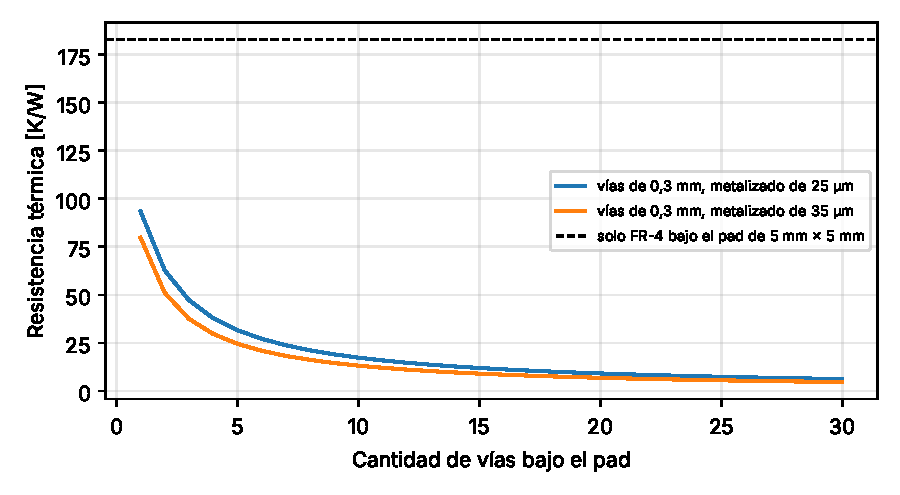
\includegraphics[width=0.85\textwidth]{resistencia_vias.pdf}
  \caption[Resistencia térmica de un conjunto de vías.]{Resistencia térmica de un conjunto de vías de \SI{0,3}{\milli\metre} en paralelo con el FR-4 bajo un pad de \SI{5}{\milli\metre}\,$\times$\,\SI{5}{\milli\metre}, en una placa de \SI{1,6}{\milli\metre} (cálculo propio).}\label{fig:termica-vias}
\end{figure}

\subsection{Camino hasta la estructura}\label{sec:termica-camino}

En una pila PC/104 no hay una placa madre: el calor llega a la estructura por los cuatro separadores de las esquinas (Capítulo~\ref{cap:pc104}). Cada separador aporta la resistencia de su cuerpo y la de las uniones atornilladas.

\subsubsection{Uniones atornilladas}

La NASA publica conductancias de uniones atornilladas que dependen del tamaño del tornillo y del par: por ejemplo, \SI{3,51}{\watt\per\kelvin} para un tornillo de 1/4--28 sobre una superficie chica y rígida y \SI{1,054}{\watt\per\kelvin} sobre superficies grandes y delgadas, y \SI{0,21}{\watt\per\kelvin} y \SI{0,105}{\watt\per\kelvin} para un tornillo 2--56 en los mismos dos casos~\cite{nasasoa}. Un ensayo de Goddard sobre una caja electrónica real en vacío mostró que los datos de catálogo, medidos en muestras chicas a presión alta, sobrestiman lo que logra una unión atornillada real, porque con tornillos solo en el perímetro el centro se separa. Los materiales de interfaz mejoraron la conductancia entre 1,2 y 28 veces según el material; el mejor (NuSil 2946) exigió unos \SI{0,5}{\milli\metre} de espesor inicial y tiene requisitos de manejo para el control de contaminación~\cite{steinfeld23}. Los rellenos térmicos comerciales que cita la NASA tienen conductividades de \SI{5}{\watt\per\metre\per\kelvin} y \SI{6}{\watt\per\metre\per\kelvin}~\cite{nasasoa}.

\subsubsection{Estimación para una pila PC/104}

Se estima la conductancia de los cuatro separadores con los datos anteriores. Hipótesis (todas propias, a confirmar con la estructura real): separadores de aluminio ($k = \SI{218}{\watt\per\metre\per\kelvin}$~\cite{guerra18}) de \SI{5}{\milli\metre} de diámetro exterior, \SI{3,2}{\milli\metre} interior y \SI{15}{\milli\metre} de largo (separación típica entre módulos, Tabla del Capítulo~\ref{cap:pc104}), con dos uniones atornilladas por separador cuya conductancia se toma como la del tornillo chico de la NASA, \SI{0,105}{\watt\per\kelvin} y \SI{0,21}{\watt\per\kelvin}. El cuerpo del separador aporta \SI{0,17}{\watt\per\kelvin}, y la Tabla~\ref{tab:termica-camino} resume el resultado.

\begin{table}[H]
  \centering
  \caption[Estimación de la conductancia de los separadores.]{Estimación (cálculo propio) del camino por cuatro separadores de aluminio, con dos uniones atornilladas cada uno.}\label{tab:termica-camino}
  \begin{tabular}{@{}*{4}{>{\centering\arraybackslash}p{3.5cm}}@{}}
    \toprule
    Conductancia por unión [W/K] & $R$ por separador [K/W] & $G$ de los cuatro [W/K] & $\Delta T$ con \SI{2}{\watt} [K] \\
    \midrule
    \num{0,105} & \num{25,0} & \num{0,160} & \num{12,5} \\
    \num{0,21}  & \num{15,5} & \num{0,259} & \num{7,7}  \\
    \bottomrule
  \end{tabular}
\end{table}

Conviene leer estos números con cuidado. Primero, las uniones dominan la resistencia: más de la mitad de $R$ está en ellas y no en el aluminio, de modo que el torque y las superficies de contacto importan más que el material del separador. Segundo, la conducción por los separadores (\num{0,16} a \SI{0,26}{\watt\per\kelvin}) es solo de 1,7 a 2,7 veces el intercambio radiante de una cara de la placa (\SI{0,095}{\watt\per\kelvin}, Sección~\ref{sec:termica-rad}), lo que confirma que no se puede ignorar la radiación interna. Tercero, esta estimación es el salto de temperatura entre la placa y la estructura, y se suma al de la placa hasta el separador y al de las vías.

\subsection{Un caso de referencia: amplificador de \SI{2}{\watt}}\label{sec:termica-guerra}

Guerra y colaboradores modelaron la electrónica de un CubeSat de \SI{10}{\centi\metre}, con tres placas, una placa de RF y cuatro varillas de aluminio como soporte, con ANSYS Icepak~\cite{guerra18}. Cada placa se modeló como diez capas de cobre en FR-4 (\SI{1,6}{\milli\metre} en total) y las varillas llevan una resistencia adicional en cada placa por la baja conductancia de contacto. La Tabla~\ref{tab:termica-guerra} resume sus resultados con un amplificador de \SI{2}{\watt}. La fuente toma \SI{80}{\celsius} como límite recomendado para ese componente~\cite{guerra18}.

\begin{table}[H]
  \centering
  \caption[Temperaturas de un amplificador de 2 W en un CubeSat.]{Resultados de Guerra y colaboradores para un amplificador que disipa \SI{2}{\watt} en un CubeSat de \SI{10}{\centi\metre}~\cite{guerra18}. El primer valor corresponde a una operación de \SI{10}{\second} cada \SI{20}{\second}, y el segundo, a \SI{5}{\second} cada \SI{20}{\second}.}\label{tab:termica-guerra}
  \begin{tabular}{@{}lc@{}}
    \toprule
    Configuración & Temperatura máxima del amplificador [$^\circ$C] \\
    \midrule
    Sin tira térmica         & 131 y 124 \\
    Con tira de grafito      & 103 y 99 \\
    \bottomrule
  \end{tabular}
\end{table}

La tira térmica es una lámina de grafito pirolítico de \SI{25}{\micro\metre} plegada en bucle, y baja unos \SI{25}{\celsius} la temperatura, pero el amplificador sigue por encima del límite de \SI{80}{\celsius}~\cite{guerra18}. Con el amplificador apagado, el componente más caliente era el procesador, a unos \SI{63}{\celsius}~\cite{guerra18}. La lección es que la etapa de potencia de RF es un punto caliente concentrado, y que un camino térmico pensado para el promedio de la placa no alcanza. Es un caso de otro satélite, con otra geometría, y no se puede trasladar directamente.

\subsection{Reglas de diseño térmico}\label{sec:termica-reglas}

La Tabla~\ref{tab:termica-reglas} resume las reglas propuestas para la placa del PI\@. Como en el capítulo anterior, se indica el origen de cada una.

\begin{table}[H]
  \centering
  \caption[Reglas de diseño térmico propuestas.]{Reglas de diseño térmico propuestas para la placa del PI y origen de cada una.}\label{tab:termica-reglas}
  \begin{tabular}{@{}>{\raggedright\arraybackslash}p{3.1cm}>{\raggedright\arraybackslash}p{7.2cm}>{\raggedright\arraybackslash}p{4.3cm}@{}}
    \toprule
    Tema & Regla & Origen \\
    \midrule
    Pad térmico & Soldar el pad del componente con al menos \SI{50}{\percent} de cobertura, y conectarlo a los planos con unión continua, sin alivio térmico. & Fuente~\cite{tislma002} \\
    Vías térmicas & Entre cinco y nueve vías bajo el pad como mínimo, de \SI{0,33}{\milli\metre} o menos, con máscara del lado del componente; más vías si la potencia lo exige. & Fuente~\cite{tislma002}; cálculo propio (Figura~\ref{fig:termica-vias}) \\
    Cobre & Planos de cobre internos continuos y de mayor espesor para repartir el calor hacia las esquinas. & Fuentes~\cite{nasasoa}; cálculo propio (Tabla~\ref{tab:termica-keq}) \\
    Camino a la estructura & Llevar el calor del componente hacia los agujeros de montaje; apretar las uniones con el torque especificado. & Cálculo propio (Tabla~\ref{tab:termica-camino}) y~\cite{steinfeld23} \\
    Punto caliente & Si la potencia es de varios vatios, prever una tira térmica o un relleno de interfaz hasta la estructura. & Fuentes~\cite{guerra18,nasasoa} \\
    Materiales de interfaz & Elegirlos con el criterio de desgasificación de la CDS\@. & Capítulo~\ref{cap:cds}; práctica \\
    Radiación & No contar con la radiación interna como sumidero: el calor debe salir por la estructura. & Cálculo propio (Sección~\ref{sec:termica-rad}) \\
    \bottomrule
  \end{tabular}
\end{table}

\verificar{si el equipo de la estructura del satélite admite una tira térmica o un relleno de interfaz entre la placa y los rieles, y qué materiales cumplen la desgasificación de la CDS}

%--------------------------------------------------------------------
\section{Blindaje y compatibilidad electromagnética}\label{sec:emi}

\subsection{Qué se necesita y qué normas existen}\label{sec:emi-normas}

En el relevamiento de la CDS del Capítulo~\ref{cap:cds} la RF aparece desde la seguridad (inhibiciones y licencias), y no se relevó un requisito numérico de emisión o inmunidad electromagnética. Para satélites en general, la norma ECSS-E-ST-20\nobreakdash-07C Rev.~2 (3 de enero de 2022), \emph{Electromagnetic compatibility}, fija requisitos detallados de sistema, condiciones de ensayo, verificación a nivel de sistema y métodos de ensayo de subsistemas y equipos, con límites informativos en un anexo~\cite{ecss2007}. Se consultó solo su página descriptiva. \verificar{los requisitos de EMC y de emisiones espurias que impondrán el proveedor de lanzamiento y la licencia de frecuencias, y si se tomará alguna norma como guía}

Para la cadena del PI hay tres necesidades concretas. La primera es que la etapa de potencia no se realimente y oscile (Sección~\ref{sec:emi-aislacion}). La segunda es que el transmisor no interfiera al receptor ni a la electrónica digital del satélite, cuya fuente de ruido son además los reguladores conmutados y los relojes. La tercera es que los armónicos y las espurias que genera el amplificador no salgan a la antena, tarea del segundo filtro de la cadena. Las dos primeras son de layout y blindaje, y son el tema de esta sección.

\subsection{Fundamentos del blindaje}\label{sec:emi-fundamentos}

La efectividad de blindaje (SE, \emph{shielding effectiveness}) es la relación en decibeles entre la señal con y sin blindaje, y se descompone en pérdida por absorción $A$ y por reflexión $R$~\cite{rosehulman}:
\begin{equation}\label{eq:emi-se}
  \mathrm{SE} = A + R, \qquad A = 8{,}69\,\frac{t}{\delta}, \qquad \delta = \sqrt{\frac{2}{\omega\mu\sigma}}, \qquad R = 20\log \frac{Z_w}{4 Z_m},
\end{equation}
con $t$ el espesor del blindaje, $\delta$ la profundidad de penetración, $Z_w \approx \SI{377}{\ohm}$ la impedancia de onda (caso de onda plana) y $Z_m = \sqrt{\omega\mu/\sigma}$ la del metal~\cite{rosehulman}. Las fuentes consultadas dan la reflexión de campo cercano (eléctrico y magnético) con constantes que no se pudieron leer, por lo que aquí solo se usa el caso de onda plana.

\begin{table}[H]
  \centering
  \caption[Blindaje de una lámina de 0,2 mm de cobre o aluminio.]{Profundidad de penetración y pérdidas de una lámina de \SI{0,2}{\milli\metre} (cálculo propio con la ecuación~\eqref{eq:emi-se}, onda plana). Conductividades: cobre \SI{5,8e7}{\siemens\per\metre} y aluminio \SI{3,7e7}{\siemens\per\metre}~\cite{rosehulman}.}\label{tab:emi-lamina}
  \begin{tabular}{@{}llcccc@{}}
    \toprule
    Material & $f$ [MHz] & $\delta$ [\si{\micro\metre}] & $Z_m$ [m$\Omega$] & $A$ [dB] & $R$ [dB] \\
    \midrule
    Cobre    & 145 & \num{5,49} & \num{4,44} & 317 & \num{86,5} \\
    Cobre    & 435 & \num{3,17} & \num{7,70} & 548 & \num{81,8} \\
    Aluminio & 145 & \num{6,87} & \num{5,56} & 253 & \num{84,6} \\
    Aluminio & 435 & \num{3,97} & \num{9,63} & 438 & \num{79,8} \\
    \bottomrule
  \end{tabular}
\end{table}

La conclusión de la Tabla~\ref{tab:emi-lamina} es que en VHF/UHF cualquier lámina metálica de décimas de milímetro es, en la práctica, un blindaje perfecto: la absorción es de cientos de decibeles y la reflexión supera los \SI{80}{\decibel}. Lo que limita la efectividad real son las aberturas y las costuras.

\subsection{Aberturas y costuras}\label{sec:emi-aberturas}

Una abertura de dimensión mayor $l$ deja pasar la señal de forma apreciable por encima de una frecuencia de corte $f_c = \SI{15000}{\mega\hertz} / l$, con $l$ en centímetros. Por debajo, la reflexión es aproximadamente $R \approx 20\log (f_c/f)$, y la absorción a través del agujero para un espesor $t$ es de $27{,}3\,t/l$ dB en una abertura rectangular~\cite{rosehulman}. Con varias aberturas iguales la efectividad cae $10\log N$ dB~\cite{rosehulman}. Como $f_c = c/2l$, la expresión de reflexión equivale a $20\log\,(\lambda/2l)$ (derivación propia). La Tabla~\ref{tab:emi-aberturas} y la Figura~\ref{fig:emi-aberturas} muestran el resultado.

\begin{table}[H]
  \centering
  \caption[Efectividad de blindaje limitada por una abertura.]{Efectividad de blindaje limitada por una abertura de dimensión mayor $l$ (cálculo propio, $R \approx 20\log (f_c/f)$ con $f_c = \SI{15000}{\mega\hertz}/l$).}\label{tab:emi-aberturas}
  \begin{tabular}{@{}rcccc@{}}
    \toprule
    $l$ [mm] & $f_c$ [GHz] & SE a \SI{145}{\mega\hertz} [dB] & SE a \SI{435}{\mega\hertz} [dB] & SE a \SI{870}{\mega\hertz} [dB] \\
    \midrule
    1  & 150  & \num{60,3} & \num{50,8} & \num{44,7} \\
    5  & 30   & \num{46,3} & \num{36,8} & \num{30,8} \\
    10 & 15   & \num{40,3} & \num{30,8} & \num{24,7} \\
    20 & 7,5  & \num{34,3} & \num{24,7} & \num{18,7} \\
    \bottomrule
  \end{tabular}
\end{table}

\begin{figure}[H]
  \centering
  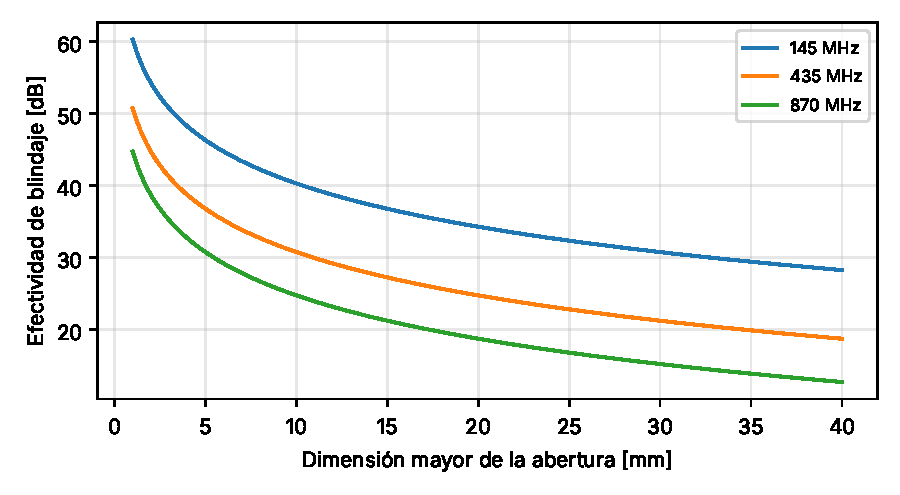
\includegraphics[width=0.85\textwidth]{se_apertura.pdf}
  \caption[Efectividad de blindaje frente al tamaño de la abertura.]{Efectividad de blindaje limitada por una abertura, según su dimensión mayor, a tres frecuencias (cálculo propio con el modelo de la Sección~\ref{sec:emi-aberturas}).}\label{fig:emi-aberturas}
\end{figure}

El modelo es una cota simple: trata la abertura como un orificio aislado en una pared plana y no incluye el espesor ni el acople con los componentes internos. Con una tapa de \SI{20}{\milli\metre} de costura abierta se obtiene a \SI{435}{\mega\hertz} unos \SI{25}{\decibel}, que es poco. Una costura fina, en cambio, se trata mejor como una hilera de aberturas de longitud igual a la separación entre contactos.

\subsection{Blindaje a nivel de placa}\label{sec:emi-placa}

El blindaje de una etapa de RF sobre la placa se realiza con una carcasa metálica soldada a un marco de cobre, unido al plano de masa inferior con una hilera de vías. El artículo de síntesis del anteproyecto de guía IEEE P2716 sobre blindajes de placa confirma que las aberturas (rendijas entre la tapa y el marco, huecos en las esquinas, orificios de ventilación) son un factor mayor en la efectividad real, y que las vías demasiado separadas pueden producir fugas, aunque no da una regla de separación~\cite{dawson23}. Una fuente divulgativa propone un paso de vías menor que $\lambda/20$, con carcasas de acero estañado o alpaca de \num{0,2} a \SI{0,3}{\milli\metre}, y da \num{40} a \SI{60}{\decibel} de efectividad para una carcasa y \num{40} a \SI{70}{\decibel} de aislación entre dos adyacentes~\cite{rfessentialsbls}. Esa fuente no cita referencias, y se la toma con cautela.

Aplicando el modelo de la Sección~\ref{sec:emi-aberturas} al espacio entre vías, un paso de $\lambda/20$ corresponde a una abertura de $l = \lambda/20$ y a una efectividad de $20\log 10 = \SI{20}{\decibel}$ exactamente, sin importar la frecuencia (cálculo propio). Es decir, $\lambda/20$ es un mínimo, y para llegar a \SI{40}{\decibel} hace falta un paso diez veces menor ($\lambda/200$). La Tabla~\ref{tab:emi-paso} muestra los números para \SI{435}{\mega\hertz} y para su segundo armónico.

\begin{table}[H]
  \centering
  \caption[Efectividad del vallado de vías según su paso.]{Efectividad estimada del vallado de vías de masa según el paso (cálculo propio, $20\log (\lambda/2p)$).}\label{tab:emi-paso}
  \begin{tabular}{@{}rcc@{}}
    \toprule
    Paso $p$ [mm] & SE a \SI{435}{\mega\hertz} [dB] & SE a \SI{870}{\mega\hertz} [dB] \\
    \midrule
    34  & \num{20,1} & \num{14,1} \\
    17  & \num{26,1} & \num{20,1} \\
    10  & \num{30,7} & \num{24,7} \\
    5   & \num{36,8} & \num{30,7} \\
    2   & \num{44,7} & \num{38,7} \\
    \bottomrule
  \end{tabular}
\end{table}

\begin{description}
  \item[Material de la carcasa.] Una carcasa de acero estañado trae el problema de los filamentos de estaño de la Sección~\ref{sec:layout-espacio}: la NASA recomienda evitar los acabados de estaño puro~\cite{brusse}. La alpaca (\emph{nickel silver}) figura como alternativa en la fuente anterior~\cite{rfessentialsbls}. \verificar{el acabado de las carcasas disponibles}
  \item[Líneas de continua y control.] La fuente divulgativa recomienda filtrar las líneas de alimentación y control en la pared del blindaje con capacitores pasantes o pines filtrados~\cite{rfessentialsbls}, para que el cable no sea la abertura.
  \item[Calor.] Una carcasa cerrada sobre el amplificador cubre justo el punto caliente; la tapa no debe ser el único camino de calor (Sección~\ref{sec:termica-camino}).
  \item[Desgasificación.] Las juntas conductoras, los absorbentes y los adhesivos del blindaje deben cumplir el criterio de TML y CVCM de la CDS (Sección~\ref{sec:layout-outgassing}). \verificar{TML y CVCM de los materiales de blindaje que se elijan}
\end{description}

\subsection{Aislación entre etapas de la cadena}\label{sec:emi-aislacion}

Un amplificador con ganancia $G$ y una trayectoria parásita de aislación $I$ entre su salida y su entrada forman un lazo de realimentación con ganancia $G - I$ (ambas en decibeles). Para que el lazo no oscile hace falta $I > G$ con un margen. Por ejemplo, con $G = \SI{20}{\decibel}$ y un margen de \SI{10}{\decibel}, la aislación necesaria es de \SI{30}{\decibel}. Es un criterio propio que no sustituye un análisis de estabilidad como el que se hace con los parámetros S del dispositivo~\cite{gonzalez}. \verificar{la ganancia de la etapa del PI y el margen de estabilidad que se exigirá}

La misma fuente divulgativa estima una aislación natural de \num{30} a \SI{50}{\decibel} para etapas separadas por más de \SI{20}{\milli\metre} y de \num{40} a \SI{70}{\decibel} con carcasas adyacentes~\cite{rfessentialsbls}. Si esos órdenes de magnitud fueran correctos, una cadena filtro--amplificador--filtro en línea recta cumpliría el ejemplo de \SI{30}{\decibel} sin blindaje, y la carcasa sería necesaria si la ganancia es mayor o si el espacio obliga a juntar etapas. Esto debe confirmarse con la ganancia real y por simulación o medición.

\subsection{Reglas de blindaje y EMC}\label{sec:emi-reglas}

\begin{table}[H]
  \centering
  \caption[Reglas de blindaje y EMC propuestas.]{Reglas de blindaje y EMC propuestas para la placa del PI y origen de cada una.}\label{tab:emi-reglas}
  \begin{tabular}{@{}>{\raggedright\arraybackslash}p{3.1cm}>{\raggedright\arraybackslash}p{7.2cm}>{\raggedright\arraybackslash}p{4.3cm}@{}}
    \toprule
    Tema & Regla & Origen \\
    \midrule
    Material & Cualquier lámina metálica de décimas de milímetro basta: las pérdidas del material no limitan. & Cálculo propio (Tabla~\ref{tab:emi-lamina}) \\
    Aberturas & Mantener las aberturas y las costuras lo más cortas posible; tratar cada costura como una hilera de aberturas. & Fuente~\cite{rosehulman}; cálculo propio \\
    Vallado de vías & Paso de vías menor que $\lambda/20$ como mínimo (\SI{20}{\decibel}), y del orden de $\lambda/100$ o menos si se busca \SI{35}{\decibel} o más. & Cálculo propio y~\cite{rfessentialsbls} \\
    Carcasa & Alpaca u otro acabado sin estaño puro, soldada al marco de cobre. & Fuentes~\cite{brusse,rfessentialsbls} \\
    Líneas de continua & Filtrar las líneas que atraviesan el blindaje. & Fuente~\cite{rfessentialsbls} \\
    Aislación & Cumplir $I > G +$ margen, con $I$ medida o simulada. & Cálculo propio \\
    Materiales & Elegir juntas y absorbentes que cumplan TML y CVCM de la CDS\@. & Capítulo~\ref{cap:cds} \\
    \bottomrule
  \end{tabular}
\end{table}

%--------------------------------------------------------------------
\section{Síntesis para el Proyecto Integrador}\label{sec:termica-sintesis}

\begin{itemize}
  \item En vacío, el calor de la etapa de potencia solo sale por conducción hasta la estructura, y la conducción de la placa es buena en el plano y mala en espesor: hacen falta vías térmicas, entre cinco y nueve como mínimo.
  \item Los separadores y sus uniones atornilladas fijan el salto de temperatura entre la placa y la estructura; con las hipótesis de este capítulo es de unos \num{8} a \SI{12}{\kelvin} para \SI{2}{\watt}.
  \item Un amplificador de \SI{2}{\watt} llegó a \SI{131}{\celsius} sin tira térmica en un caso publicado, por lo que la potencia que disipe el PI y su límite de temperatura son datos de entrada críticos.
  \item En VHF/UHF el material del blindaje no es el problema; lo son las aberturas, las costuras y el paso de las vías. Un paso de $\lambda/20$ da solo \SI{20}{\decibel}.
  \item Los materiales de interfaz, las juntas y los acabados deben cumplir la desgasificación de la CDS y evitar el estaño puro.
\end{itemize}

\chapter{Conclusiones}
\label{cap:conclusiones}


% ---------- Bibliografía ----------
\printbibliography[heading=bibintoc,title={Bibliografía}]

% ---------- Anexos ----------
\appendix
% \input{anexos/A_ejemplo}

\end{document}
